%# -*- coding: utf-8-unix -*-
%%==================================================

\chapter{真题讲解}
\label{chap21}

杭电真题只有近三年的价值最高,其他的如果时间不足可以不做☆ \newline
对应2020年考研,2017,2018,2019三年最为重要.\newline
因为有一些题目出的模棱两可,实在不必深究,这种题目会越来越少,越来越逼近408这就是趋势。\newline
注解:QU 表示此题有疑问\newline
\begin{itemize}[noitemsep,topsep=0pt,parsep=0pt,partopsep=0pt]
	\item 2017数据结构真题(150分)
	\item 2017数据结构真题答案
\end{itemize}


\section{真题}
一、判断题(T正确,F错误。本大题共6小题,每小题1分,本大题共6分)\newline
1. 判断带头结点的非空循环单链表(头指针为L)中指针p所指节点是最后一个元素节点的条件是:p->nxt == L. (  )\newline
2. 对于频繁的插入、删除而言,线性表的链式存储由于顺序存储.(  )\newline
3. 二叉树是一颗结点的度最大为2的树.(  )\newline
4. 哈夫曼树中节点个数一定是奇数.(  )\newline
5. 在二叉树中序遍历序列中,任意一个节点均处在其左孩子节点的后面.(  )\newline
6. 由树节点的先根序列和后跟序列可以唯一地确定一棵树.(  )\newline
~\\

二、 单项选择题(本大题共10空,每空1分,本大题共10分)\newline
1. 在一个长度为n的顺序表中删除第i个元素,需要向前移动 (  ) 个元素。\newline
A. n-i       B. n-i+1    C. n-i-1   D. i+1\newline
2. 先后5个数字1,2,3,4,5, 依次顺序进入栈, 可以得到 (  ) 的出栈。\newline
A. 3,4,5,1,2           B. 2,3,1,3,4\newline
C. 3,5,4,2,1           D. 1,3,5,2,4\newline
3. 假定在一棵二叉树中,度为2的结点数为15,度为1的结点数为30,则叶子结点数为(  )个。\newline
A. 15   B. 16    C. 17  D. 47 \newline
4. 若需要在$O(nlog_2n)$的时间内完成对一组数据的排序,且要求排序是稳定的,则可选择的排序方法是(  )。\newline
A. 快速排序    B. 堆排序  C. 归并排序  D. 直接插入排序 \newline
5. 下面有向图所示的拓扑排序一种可能的结果序列是(  )。\newline
A. 125634     B.  516234    C.  123456    D. 521643\newline
\begin{figure}[H]
	\centering  % 环境中的内容居中排版
	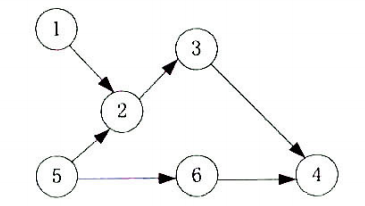
\includegraphics[scale=0.3]{example/chapter21/Annotation2019-08-24114921.png}
\end{figure}
6. 设计一个判别表达式中括号是否配对的算法,采用(  ) 数据结构最佳.\newline
A. 顺序表    B. 链表   C. 队列    D. 栈  \newline
7. 关键路径是指在只有一个源点和一个汇点的有向无环网中源点至汇点(   )的路径\newline
A. 弧的数目最多   B.  弧的数目最少   C.  权值之和最大    D. 权值之和最小\newline
8. 一个序列有10000个元素,若指向得到其中前10个最小元素,则最好采用(  ) 方法。\newline
A. 快速排序  B. 插入排序  C. 堆排序  D. 归并排序 \newline
9. 下列排序方法中 (  ) 具有最好的平均性能;当待排序序列的关键词次序为倒序是,且需为之进行正序排序,则下列排序中 (  ) 为佳。\newline
A. 堆排序  B. 快速排序  C. 直接插入排序  D. 简单选择排序 \newline

三、填空图 (本大题共24空, 每空2分, 本大题共48分)\newline
1. 一个算法具有5个特性:\_\_\_(1)\_\_\_、 \_\_\_(2)\_\_\_、 \_\_\_(3)\_\_\_、有0个或多个输入、有一个或多个输出。
2. 设循环队列的容量为70,front指向队头, rear指向队尾的下一个位置。现经过一些列的入队和出队操作后,front为20, rear为 11, 则队列中元素的个数为\_\_\_(4)\_\_\_.\newline
3. 散列存储的基本思想是由 \_\_\_(5)\_\_\_确定记录的存储地址。\newline
4. 设栈S和队列Q的初始状态为空,元素e1,e2,e3,e4,e5,e6依次通过栈S,一个元素出栈后即进入队列Q,若6个元素出队的序列是e2,e4,e3,e6,e5,e1,则栈的容量至少应该是\_\_\_(6)\_\_\_. \newline
5. 对广义表L=((a,b), ((c,d),(e,f)))执行head(tail(head(tail(L))))操作的结果是\_\_\_(7)\_\_\_. \newline
6. 
\begin{lstlisting}[basicstyle=\small\ttfamily, caption={}, numbers=none]
void fun(int n){
	int i = 0; s=0;
	while(s<n){
		++i;
		s=s+i;
	}
}该算法的时间复杂度为___(8)___.
\end{lstlisting}
7. 若有序表中关键字序列为: 15,20, 25, 30, 35,40, 45, 50, 55, 60, 65.对其进行折半查找,则在等概率情况下,查找成功时的平均查找程度是
\_\_\_(9)\_\_\_. 查找65时需进行\_\_\_(10)\_\_\_次比较。\newline
8. 已知Hash函数为H(K) = K mod 13, 散列地址为 0 —— 14,用开放地址法解决冲突,选取增量序列为线性探测再散列, 关键字23,34,56,24,75,12,49,52,36,95依次插入到散列表中,则平均成功的查找长度为\_\_\_(11)\_\_\_、平均失败的查找长度为\_\_\_(12)\_\_\_\newline
9. 假设用于通讯的电文仅由6个字符组成,字母在电文中出现的频率分别为35, 5, 12, 8, 25, 15. 依照哈夫曼树构建算法, 若为这66个字母设计哈夫曼编码,则频率为5的字符编码是\_\_\_(13)\_\_\_, 该哈夫曼树高度为\_\_\_(14)\_\_\_, 带权路径长度为\_\_\_(15)\_\_\_。\newline
10. 循环队列定义如下:请在航线上填写合适的语句, 实现进队列和出队列的操作。
\begin{lstlisting}[basicstyle=\small\ttfamily, caption={}, numbers=none]
#define MAXSIZE 5;
typedef int elemtype;
struct sequeue
{
	elemtype queue[MAXSIZE];
	int front, rear;
};
Status enqueue(sequeue &q, elemtype x)
{
	if(___(16)___) return ERROR;//队列满
	q.queue[q.rear] = x;
	q.rear = ____(17)____;
	return OK;
}
Status dlqueue(sequeue &q, elemtype &x)
{
	if (___(18)___) return EROOR;// 队列空
	x = q.queue[q.front];
	q.front=___(19)___;
	return OK;
}
\end{lstlisting}
11. 二叉树用二叉链表的结构描述,函数depth实现返回二叉树的高度,请在空格处将算法补充完整。
\begin{lstlisting}[basicstyle=\small\ttfamily, caption={}, numbers=none]
typedef struct node{
	char data;
	struct node *lchild;
	struct node *rchild;
}NODE;
int depth(NODE *t){
	int hl, hr;
	if (t == NULL)
		return 0;
	else{
		hl = depth(t->lchild);
		hr=___(20)___;
		if(___(21)___)
			return hl+1;
		else
			return hr+1;
	}
}
\end{lstlisting}

12. 请在横线上填写合适的语句,完成折半插入算法。\newline

\begin{lstlisting}[basicstyle=\small\ttfamily, caption={}, numbers=none]
void BInsertSort(int R[])
{
	int i, j, low, high, m;
	for(i = 2; i<=N; ++i){
		R[0] = R[i];
		low = l;
		high = i - 1;
		while(___(22)___){
			___(23)___;
			if(R[0]<R[m]) high = m - 1;
			else low = m + 1;
		}
		for(j = i -1; j>=high+1;--j) R[j+1] = R[j];
		___(24)___;
	}
}
\end{lstlisting}

四、算法阅读题(阅读以下算法代码, 指出算法的功能。 本大题共4小题,每小题5分, 本大题共20分)\newline
1) 第一题代码:\newline
\begin{lstlisting}[basicstyle=\small\ttfamily, caption={}, numbers=none]
void A1(Node *T, int m){
	InitStack(S);
	itn i;
	if (T == NULL) return;
	Push(S, T);
	while(!StackEmpty(S)){
		Pop(S,T);
		printf("%c", T->data);
		for (i = m - 1; i>=0; i--)
			if(T->child[i] != NULL)
				Push(S, T->child[i]);
	}
}
\end{lstlisting}

2) 第二题代码:\newline
\begin{lstlisting}[basicstyle=\small\ttfamily, caption={}, numbers=none]
int A2(char a[], char b[]){
	int n,m,i,j;
	m = strlen(a);
	n = strlen(b);
	for(i =0; i<=n-m; i++){
		for(j=0; j<m&&a[i+j]==b[j];j++)
			if(j == m)
				return i+1;
	}
	return 0;
}
\end{lstlisting}

3) 第三题代码:\newline
\begin{lstlisting}[basicstyle=\small\ttfamily, caption={}, numbers=none]
#define M 30
int A3(int v, int t[]){
	int a, i;
	a = fun(v);
	for(i = 0; i<M && t[(a+i)%M]!=0; i++){
		if(t[(a+i)%M] == v)
			return (a+i)%M;
	}
	return -1;
}
\end{lstlisting}
4) 第四题代码:\newline
\begin{lstlisting}[basicstyle=\small\ttfamily, caption={}, numbers=none]
void A4(int a[], int n, int d[], int t){
	int i,j,k,y;
	for(i=0; i<t; i++){
		for(j=d[i]; j<n; j++){
			y = a[j];
			for(k=j-d[i]; k>=0 && y<a[k]; k-=d[i])
				a[k+d[i]] = a[k];
			a[k+d[i]] = y;
		}
	}
}

\end{lstlisting}

五、图示问答图(本大题共5小题, 每小题6分, 本大题共 30 分)\newline
1. 已知二叉树的先序、中序、后序遍历的结果分别如下,请 
1) 画出这棵二叉树,
2) 补齐遍历中的空白处,
3) 画出中序线索化二叉树形。
先序序列: \_ B \_ F \_ I C E H \_ G
中序序列: D \_ K F I A \_ E J C G
后序序列: D K I F \_ H J E G C A

2. 将下图所示的森林转换成一棵二叉树,并画出这棵二叉树的顺序存储结构。\newline
\begin{figure}[H]
	\centering  % 环境中的内容居中排版
	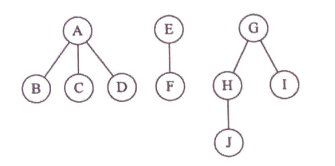
\includegraphics[scale=0.8]{example/chapter21/2019-09-10112932.png}
\end{figure} 

3. 请对下列带权无向图,按普里姆(Prim)算法求其最小生成树。(给出求解过程)\newline
\begin{figure}[H]
	\centering  % 环境中的内容居中排版
	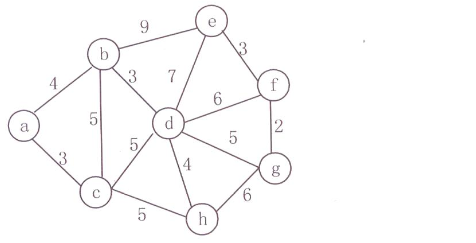
\includegraphics[scale=0.8]{example/chapter21/2019-09-10113325.png}
\end{figure} 

4. 已知图G如下所示,求从顶点a到其余各顶点的最短路径。(给出求解过程)\newline
\begin{figure}[H]
	\centering  % 环境中的内容居中排版
	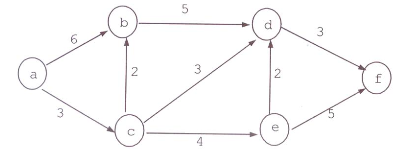
\includegraphics[scale=0.8]{example/chapter21/2019-09-10124650.png}
\end{figure} 

5. 设数据元素的关键字序列为(20, 30, 15, 45, 78, 65, 25, 60)依次插入这些元素,创建一颗平衡二叉排序树(AVL 树),请逐一画出每插入一个元素后的AVL树的形态。\newline

六、算法设计题(本大题共三小题, 第一小题10分, 第二小题12分, 第三小题14分, 本大题共36分)\newline
1. 二叉树的节点类型定义为\newline

\begin{lstlisting}[basicstyle=\small\ttfamily, caption={}, numbers=none]
typedef struct node{
	char data;
	struct node *lchild;
	struct node *rchild;
}NODE;
\end{lstlisting}
设计以非递归的方式实现对二叉树先序遍历的算法。\newline

2. 假设待排序的n个元素存放在数据a[1],......,a[n]中,利用堆排序算法对n个元素进行升序排序。\newline
1) 请描述堆排序算法步骤;\newline
2) 写出堆排序的代码; \newline

3. 采用邻接表存储结构, 编写一个判别无向图中任意给定的两个顶点之间是否存在一条长度为K的简单路径的算法。注:简单路径是指其顶点序列中不含有重现的顶点。\newline


\section{答案}
一、判断题(T正确,F错误。本大题共6小题,每小题1分,本大题共6分)\newline
1. 判断带头结点的非空循环单链表(头指针为L)中指针p所指节点是最后一个元素节点的条件是:p->next == L. (  )\newline
解:T\newline
正确应该是: p!=L \&\& p->next == L \newline
2. 对于频繁的插入、删除而言,线性表的链式存储由于顺序存储.(  )\newline
解:T\newline
顺序存储插入,要频繁移动后面的元素,链表不会,所以是T.\newline
3. 二叉树是一颗结点的度最大为2的树.(  )\newline
解:F\newline
二叉树左右子树不可交换,所以和结点度最大为二的树有本质差别.\newline
4. 哈夫曼树中节点个数一定是奇数.(  )\newline
解:T\newline
哈夫曼树结点个数是 2N-1, N 表示有多少个数参与构建了这颗哈夫曼树.\newline
5. 在二叉树中序遍历序列中,任意一个节点均处在其左孩子节点的后面.(  )\newline
解:T\newline
LDR中序遍历就是有这个特性\newline
6. 由树结点的先根序列和后跟序列可以唯一地确定一棵树.(  )\newline
解:F\newline
参考链接\url{https://www.zybang.com/question/07bd009430f3d3fc84a4abb6b027840e.html}只要知道中根遍历顺序,再加上其余两个遍历中任意一个都可以唯一确定一个二叉树,
如果不知道中根遍历顺序,则无法确定.\newline

二、 单项选择题(本大题共10空,每空1分,本大题共10分)\newline
1. 在一个长度为n的顺序表中删除第i个元素,需要向前移动 (  ) 个元素。\newline
A. n-i       B. n-i+1    C. n-i-1   D. i+1\newline
解: A \newline
举例法:10个元素\{1,2,3,4,5,6,7,8,9,10\},删去第5个元素,移动6,7,8,9,10。移动5个元素。所以是n-i
2. 先后5个数字1,2,3,4,5, 依次顺序进入栈, 可以得到 (  ) 的出栈。\newline
A. 3,4,5,1,2           B. 2,4,1,3,5\newline
C. 3,5,4,2,1           D. 1,3,5,2,4\newline
解: C\newline
A. 1 push 2 push 3 push 3 out 4 push 4 out 5 push 5 out 2 push 2 out 1 push 1 out , $\therefore$ error\newline 
B. 1 push 2 push 2 out 3 push 4 push 4 out , $\therefore$ error\newline
C. 1 push 2 push 3 push 3 out 4 push 5 push 5 out 4 out 2 out 1 out, $\therefore$ 是对的.\newline
D. 略
3. 假定在一棵二叉树中,度为2的结点数为15,度为1的结点数为30,则叶子结点数为(  )个。\newline
A. 15   B. 16    C. 17  D. 47 \newline
解:B \newline
$N2 + N1 + N0 = N1 + 2*N2 + 1$ 公式 15 + 30 + N0 = 30 + 30 + 1 $\therefore$ N0 = 61 -45 = 16
4. 若需要在$O(nlog_2n)$的时间内完成对一组数据的排序,且要求排序是稳定的,则可选择的排序方法是(  )。\newline
A. 快速排序    B. 堆排序  C. 归并排序  D. 直接插入排序 \newline
解: C \newline
排序稳定,堆排序和归并排序的时间复杂度$nlog_2n$.但是堆排序是不稳定排序,因为不能保证两个一样的数据不会交换位子。所以是归并排序\newline
5. 下面有向图所示的拓扑排序一种可能的结果序列是(  )。\newline
A. 125634     B.  516234    C.  123456    D. 521643\newline
\begin{figure}[H]
	\centering  % 环境中的内容居中排版
	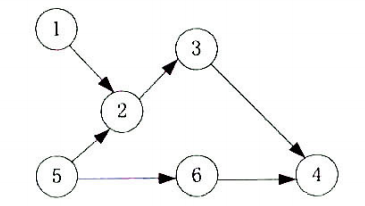
\includegraphics[scale=0.3]{example/chapter21/Annotation2019-08-24114921.png}
\end{figure}
解: \newline
A. 1 后面肯定是5,$\therefore$ ERROR \newline
B. 5,1,6,2,3,4 成立$\therefore$ RIGHT \newline
C.D. 略
6. 设计一个判别表达式中括号是否配对的算法,采用(  ) 数据结构最佳.\newline
A. 顺序表    B. 链表   C. 队列    D. 栈  \newline
解: D \newline
参看 严蔚敏的书,严老师设计了一个使用栈来计算的算法 \newline
7. 关键路径是指在只有一个源点和一个汇点的有向无环网中源点至汇点(   )的路径\newline
A. 弧的数目最多   B.  弧的数目最少   C.  权值之和最大    D. 权值之和最小\newline
解: C \newline
考虑一个v1 节点 到 v2 节点,其中有两条路径,一条5, 一条 3 ,如果3,那么 v2 活动是否可以开始了呢?不行,因为 v2 依赖路径为5的事件完成才能继续。\newline
8. 一个序列有10000个元素,若指向得到其中前10个最小元素,则最好采用(  ) 方法。\newline
A. 快速排序  B. 插入排序  C. 堆排序  D. 归并排序 \newline
解: C \newline
参考链接 \url{https://zhidao.baidu.com/question/1991976779144389267.html} \newline 
9. 下列排序方法中 (  ) 具有最好的平均性能;当待排序序列的关键词次序为倒序是,且需为之进行正序排序,则下列排序中 (  ) 为佳。\newline
A. 堆排序  B. 快速排序  C. 直接插入排序  D. 简单选择排序 \newline
解: B D\newline
快速排序拥有最好的平均性能,时间复杂度相同但是,快排拥有最小的系数\newline
简单选择排序 参考链接 \url{https://www.docin.com/p-965521183.html} 第13 题。

二、 单项选择题(本大题共10空,每空1分,本大题共10分)\newline
1. 在一个长度为n的顺序表中删除第i个元素,需要向前移动 (  ) 个元素。\newline
A. n-i       B. n-i+1    C. n-i-1   D. i+1\newline
2. 先后5个数字1,2,3,4,5, 依次顺序进入栈, 可以得到 (  ) 的出栈。\newline
A. 3,4,5,1,2           B. 2,3,1,3,4\newline
C. 3,5,4,2,1           D. 1,3,5,2,4\newline
3. 假定在一棵二叉树中,度为2的结点数为15,度为1的结点数为30,则叶子结点数为(  )个。\newline
A. 15   B. 16    C. 17  D. 47 \newline
4. 若需要在$O(nlog_2n)$的时间内完成对一组数据的排序,且要求排序是稳定的,则可选择的排序方法是(  )。\newline
A. 快速排序    B. 堆排序  C. 归并排序  D. 直接插入排序 \newline
5. 下面有向图所示的拓扑排序一种可能的结果序列是(  )。\newline
A. 125634     B.  516234    C.  123456    D. 521643\newline
\begin{figure}[H]
	\centering  % 环境中的内容居中排版
	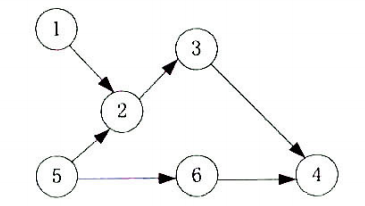
\includegraphics[scale=0.3]{example/chapter21/Annotation2019-08-24114921.png}
\end{figure}
6. 设计一个判别表达式中括号是否配对的算法,采用(  ) 数据结构最佳.\newline
A. 顺序表    B. 链表   C. 队列    D. 栈  \newline
7. 关键路径是指在只有一个源点和一个汇点的有向无环网中源点至汇点(   )的路径\newline
A. 弧的数目最多   B.  弧的数目最少   C.  权值之和最大    D. 权值之和最小\newline
8. 一个序列有10000个元素,若指向得到其中前10个最小元素,则最好采用(  ) 方法。\newline
A. 快速排序  B. 插入排序  C. 堆排序  D. 归并排序 \newline
9. 下列排序方法中 (  ) 具有最好的平均性能;当待排序序列的关键词次序为倒序是,且需为之进行正序排序,则下列排序中 (  ) 为佳。\newline
A. 堆排序  B. 快速排序  C. 直接插入排序  D. 简单选择排序 \newline

三、填空图 (本大题共24空, 每空2分, 本大题共48分)\newline
1. 一个算法具有5个特性:\_\_\_(1)\_\_\_、 \_\_\_(2)\_\_\_、 \_\_\_(3)\_\_\_、有0个或多个输入、有一个或多个输出。\newline
解:\newline
有穷性,确定性,可行性\newline
2. 设循环队列的容量为70,front指向队头, rear指向队尾的下一个位置。现经过一些列的入队和出队操作后,front为20, rear为 11, 则队列中元素的个数为\_\_\_(4)\_\_\_.\newline
解:\newline
应该有61元素 (Q.rear - Q.front + MAXSIZE) \% MAXISZE \newline 
[0,1,...10, , , , , 20,21,22,...,69] \newline
3. 散列存储的基本思想是由 \_\_\_(5)\_\_\_确定记录的存储地址。\newline
关键码值\newline
4. 设栈S和队列Q的初始状态为空,元素e1,e2,e3,e4,e5,e6依次通过栈S,一个元素出栈后即进入队列Q,若6个元素出队的序列是e2,e4,e3,e6,e5,e1,则栈的容量至少应该是\_\_\_(6)\_\_\_. \newline
解:\newline 
应该是 3 手动模拟\newline 
5. 对广义表L=((a,b), ((c,d),(e,f)))执行head(tail(head(tail(L))))操作的结果是\_\_\_(7)\_\_\_. \newline
解:\newline
tail(L) = (((c,d),(e,f))) = L1 \newline
head(L1) = ((c,d),(e,f)) = L2 \newline
tail(L2) = ((e,f)) = L3 \newline
head(L3) = (e,f) = L4 \newline
答案是   (e,f) \newline

6. 
\begin{lstlisting}[basicstyle=\small\ttfamily, caption={}, numbers=none]
void fun(int n){
	int i = 0; s=0;
	while(s<n){
	++i;
	s=s+i;
	}
}该算法的时间复杂度为___(8)___.
\end{lstlisting}
解:\newline
可以看出计算的流程是简单的等差数列求和\newline
令经过t步骤函数停止\newline
1+2+3+4+5...+t >= n\newline
(1+t)*t / 2 >= n\newline
t -> sqrt(n) 答案是 O(n)  取消相关常数项的系数\newline
7. 若有序表中关键字序列为: 15, 20, 25, 30, 35,40, 45, 50, 55, 60, 65.对其进行折半查找,则在等概率情况下,查找成功时的平均查找长度是
\_\_\_(9)\_\_\_. 查找65时需进行\_\_\_(10)\_\_\_次比较。\newline
解:\newline
3\newline
15,20,25,30,35,40,45,50,55,60,65\newline
3,4,2,3,4,1,3,4,2,3,4   和为  33 / 11 = 3\newline
4次\newline
8. 已知Hash函数为H(K) = K mod 13, 散列地址为 0 —— 14,用开放地址法解决冲突,选取增量序列为线性探测再散列, 关键字23,34,56,24,75,12,49,52,36,95依次插入到散列表中,则平均成功的查找长度为\_\_\_(11)\_\_\_、平均失败的查找长度为\_\_\_(12)\_\_\_\newline
解:\newline
\begin{tabular}{|c|c|c|c|c|c|c|c|c|c|c|c|c|c|c|}% 通过添加 | 来表示是否需要绘制竖线
	\hline  % 在表格最上方绘制横线
	0 & 1 & 2 & 3 & 4 & 5 & 6 & 7 & 8 & 9 & 10 & 11 & 12 & 13 & 14 \\
	\hline  %在第一行和第二行之间绘制横线
	52(1) & 36(7) & 92(2) &   & 56(1) &   &   &   & 34(1) &   & 23(1) & 24(1) & 75(3) & 12(2) & 49(5) \\
	\hline
	4 & 3 & 2 &  1 & 2 & 1 &  1 &  1 & 2 & 1 & 9 & 8 & 7 & 6 &  5  \\
	\hline % 在表格最下方绘制横线
\end{tabular}

\begin{lstlisting}[basicstyle=\small\ttfamily, caption={}, numbers=none]
23 % 13 = 10
34 % 13 = 8   
56 % 13 = 4
24 % 13 = 11
75 % 13 = 10  冲突  (10 + 1 ) % 15=11 冲突 (10 + 2)% 15 = 12
12 % 13 = 12  冲突  (12 + 1) % 15 =13 
49 % 13 = 10  冲突   (10 + 1 ) % 15=11 冲突 (10 + 2)% 15 = 12 冲突 (10 + 3) % 15 =13 冲突  (10 + 4) % 15 = 14
52 % 13 = 0 
36 % 13 = 10  冲突   (10 + 1 ) % 15=11 冲突 (10 + 2)% 15 = 12 冲突 (10 + 3) % 15 =13 冲突  (10 + 4) % 15 = 14 (10 + 5) % 15 = 0 冲突(10 + 6)% 15 = 1 
92 % 13 = 1 (1+1)% 15 = 2
\end{lstlisting}

\rule[-10pt]{20cm}{0.05em}

\begin{flalign}
1 + 7 + 2 + 1 + 1 + 1+ 1 + 3 + 2 + 5 &= 24  (\mbox{查找次数}) &&\\
24 / 10 &=2.4  (\mbox{平均查找长度}) 
\end{flalign}


对于0地址的元素要查找0,1,2,3这几个元素才知道会不会失败,第三个是空元素,所以失败了
对于1地址的元素要查找1,2,3这几个元素才知道会不会失败,第3个元素是空元素,所以失败了
以此类推
因为 mod 13 只用看  0 - 12空间里面的错误 
\begin{flalign}
(4+ 3 + 2 + 1 + 2 + 1 + 1 +1 + 2 + 1 + 9 + 8 + 7 ) &= 42 &&\\ 
ASL_{\mbox{失败}} &= 42 / 13 
\end{flalign}
9. 假设用于通讯的电文仅由6个字符组成,字母在电文中出现的频率分别为35, 5, 12, 8, 25, 15. 依照哈夫曼树构建算法, 若为这66个字母设计哈夫曼编码,则频率为5的字符编码是\_\_\_(13)\_\_\_, 该哈夫曼树高度为\_\_\_(14)\_\_\_, 带权路径长度为\_\_\_(15)\_\_\_。\newline
解:\newline
\begin{figure}[H]
	\centering  % 环境中的内容居中排版
	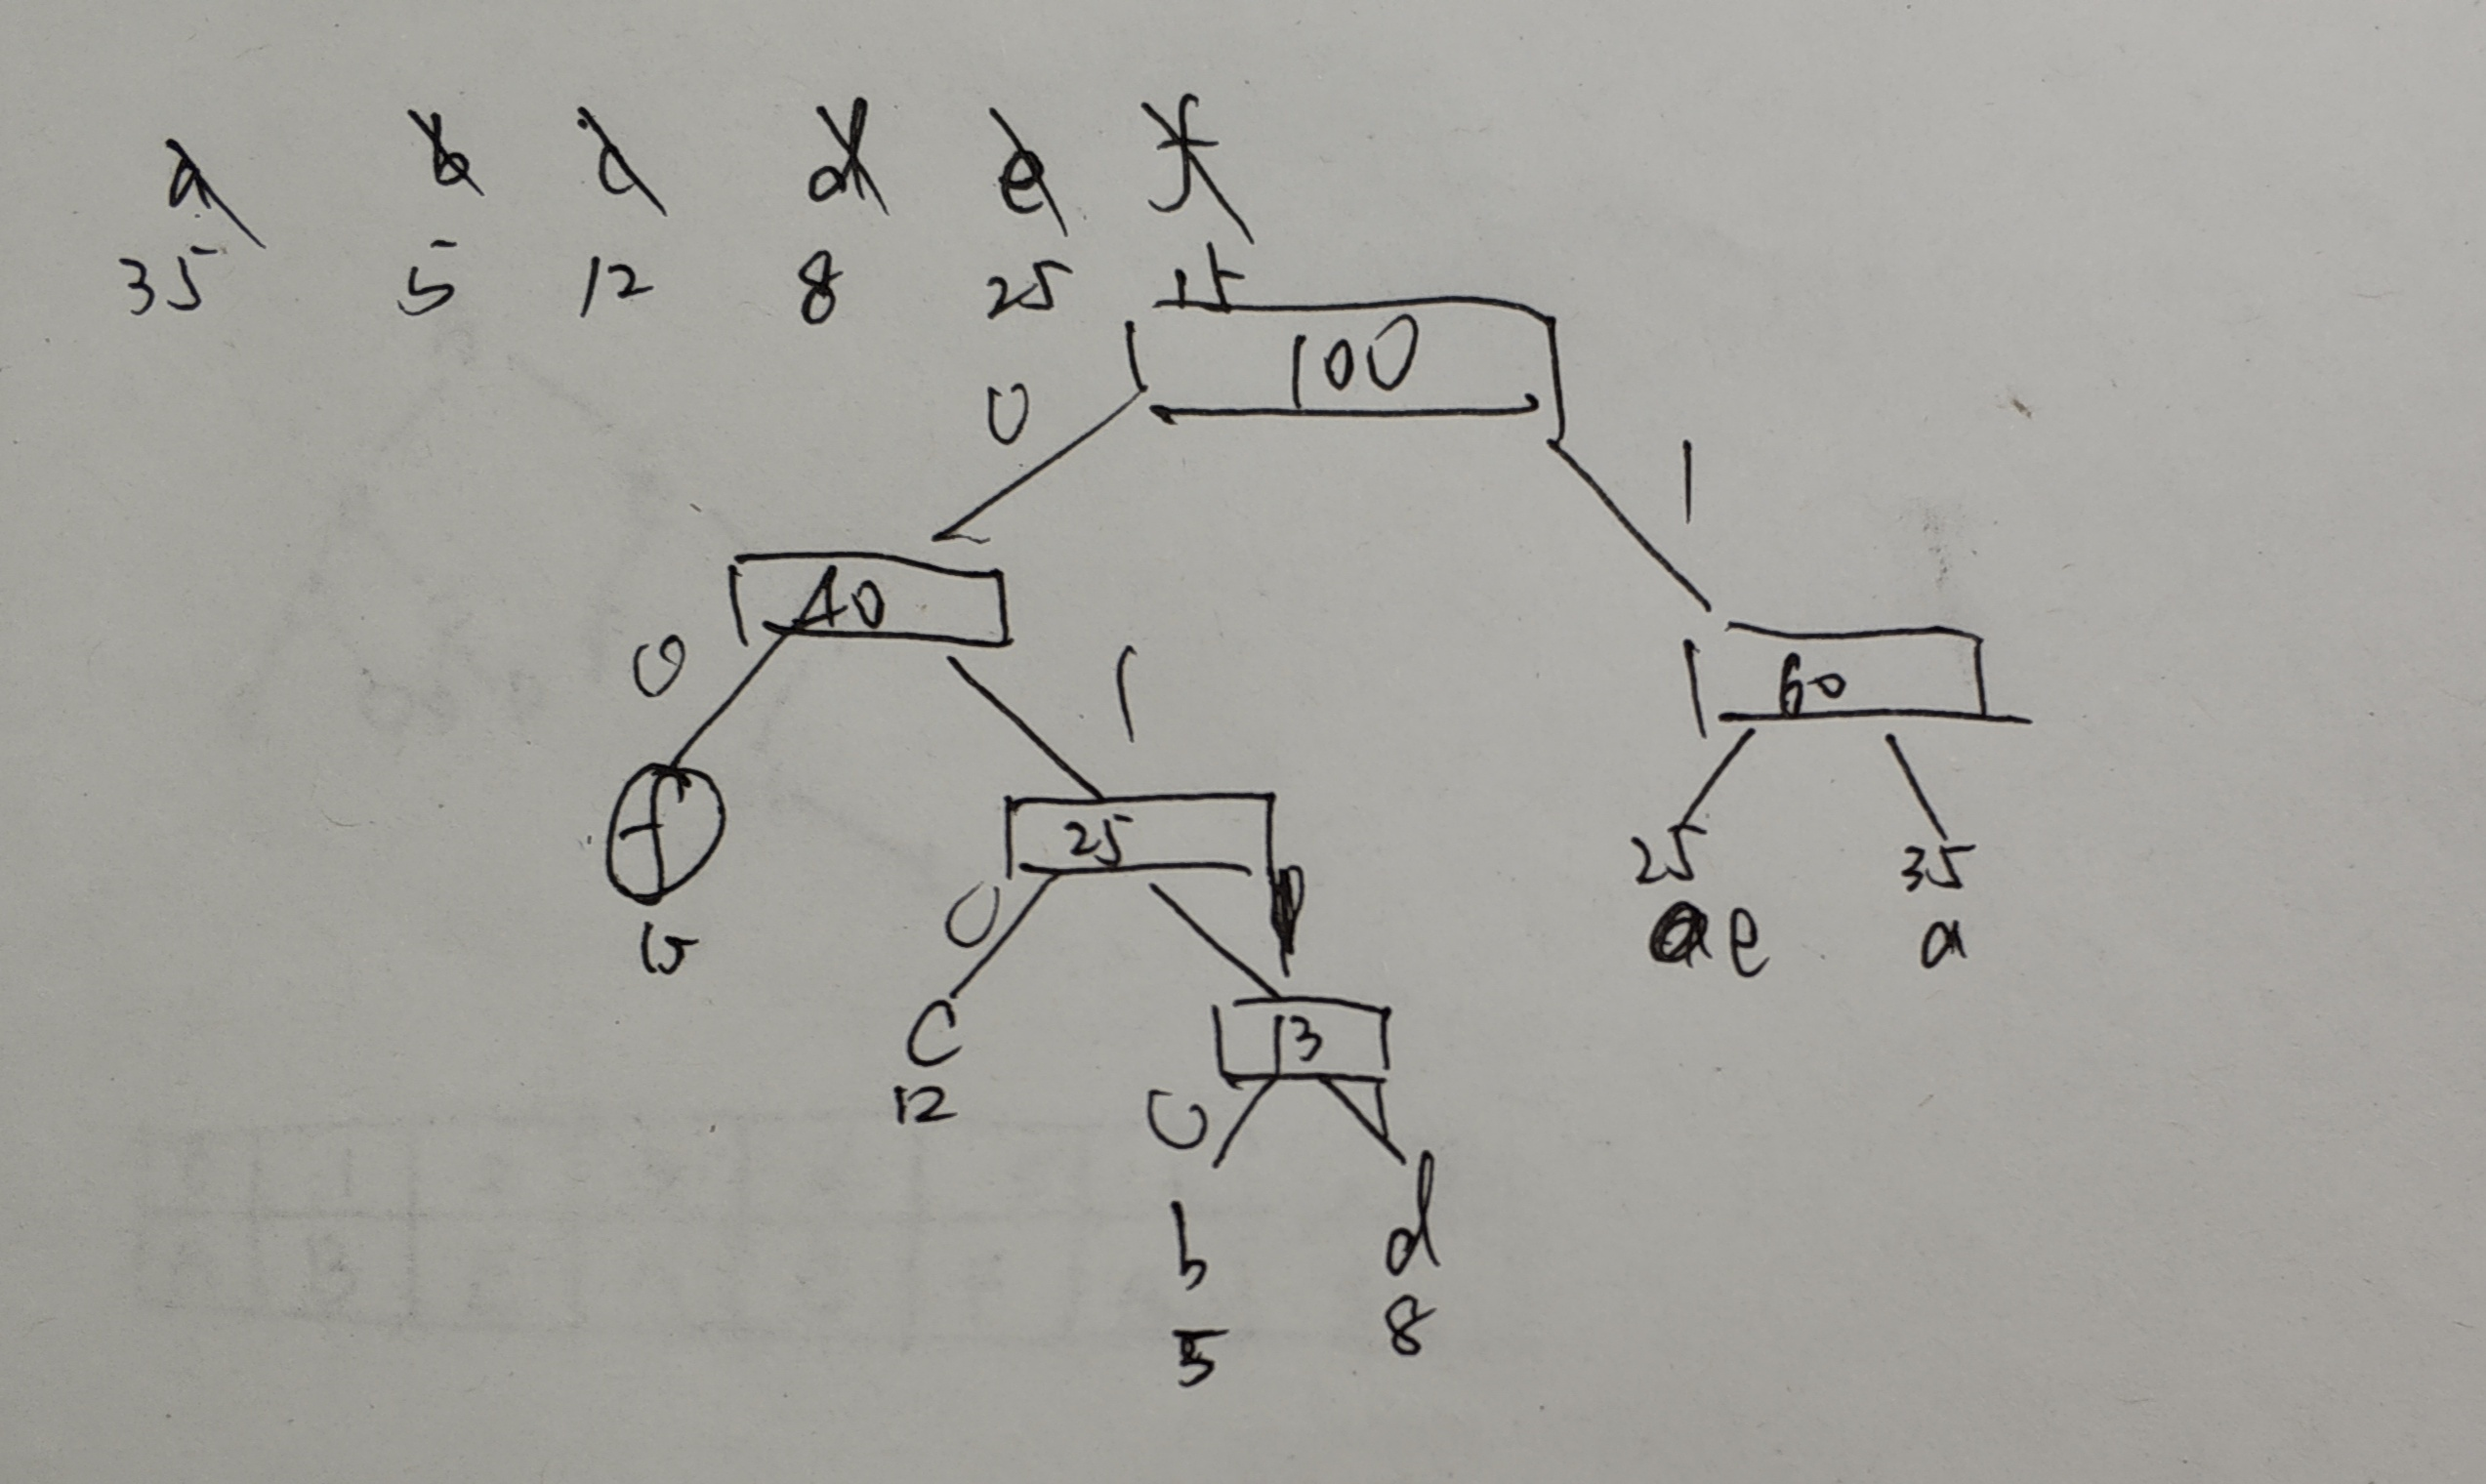
\includegraphics[scale=0.1]{example/chapter3/IMG_20181128_112049.png}
\end{figure}
~\\
5的编码 0110(不唯一,最好遵守左小右大,左0右1)\newline
高度   5\newline
$$WPL = (5*4 +8*4 + 12*3 + 15 *2 + 25 * 2 + 35 *2)=238 $$
10. 循环队列定义如下:请在航线上填写合适的语句, 实现进队列和出队列的操作。
\begin{lstlisting}[basicstyle=\small\ttfamily, caption={}, numbers=none]
#define MAXSIZE 5;
typedef int elemtype;
struct sequeue
{
	elemtype queue[MAXSIZE];
	int front, rear;
};
Status enqueue(sequeue &q, elemtype x)
{
	if(___(16)___) return ERROR;//队列满
	q.queue[q.rear] = x;
	q.rear = ____(17)____;
	return OK;
}
Status dlqueue(sequeue &q, elemtype &x)
{
	if (___(18)___) return EROOR;// 队列空
	x = q.queue[q.front];
	q.front=___(19)___;
	return OK;
}
\end{lstlisting}
解:\newline
16: (q.rear + 1) \% MAXSIZE == q.front\newline
17: (q.rear + 1) \% MAXSIZE \newline
18: q.front == q.rear \newline
19: (q.front + 1) \% MAXSIZE \newline 
11. 二叉树用二叉链表的结构描述,函数depth实现返回二叉树的高度,请在空格处将算法补充完整。
\begin{lstlisting}[basicstyle=\small\ttfamily, caption={}, numbers=none]
typedef struct node{
	char data;
	struct node *lchild;
	struct node *rchild;
}NODE;
int depth(NODE *t){
	int hl, hr;
	if (t == NULL)
		return 0;
	else{
		hl = depth(t->lchild);
		hr=___(20)___;
		if(___(21)___)
			return hl+1;
		else
			return hr+1;
	}
}
\end{lstlisting}
解:\newline
20:depth(t->rchild); \newline
21:hl > hr \newline
12. 请在横线上填写合适的语句,完成折半插入算法。\newline

\begin{lstlisting}[basicstyle=\small\ttfamily, caption={}, numbers=none]
void BInsertSort(int R[])
{
	int i, j, low, high, m;
	for(i = 2; i<=N; ++i){
		R[0] = R[i];
		low = l;
		high = i - 1;
		while(___(22)___){
			___(23)___;
			if(R[0]<R[m]) high = m - 1;
			else low = m + 1;
		}
		for(j = i -1; j>=high+1;--j) R[j+1] = R[j];
		___(24)___;
	}
}
\end{lstlisting}
22: low <= high\newline
23: m = (low + high) / 2;\newline
24: R[high+1] = R[0]\newline
四、算法阅读题(阅读以下算法代码, 指出算法的功能。 本大题共4小题,每小题5分, 本大题共20分)\newline
1) 第一题代码:\newline
\begin{lstlisting}[basicstyle=\small\ttfamily, caption={}, numbers=none]
void A1(Node *T, int m){
	InitStack(S);
	int i;
	if (T == NULL) return;
	Push(S, T);
	while(!StackEmpty(S)){
		Pop(S,T);
		printf("%c", T->data);
		for (i = m - 1; i>=0; i--)
			if(T->child[i] != NULL)
				Push(S, T->child[i]);
	}
}
\end{lstlisting}
解:\newline
树的先根遍历\newline

2) 第二题代码:\newline
\begin{lstlisting}[basicstyle=\small\ttfamily, caption={}, numbers=none]
int A2(char a[], char b[]){
	int n,m,i,j;
	m = strlen(a);
	n = strlen(b);
	for(i =0; i<=n-m; i++){
		for(j=0; j<m&&a[i+j]==b[j];j++)
			if(j == m)
				return i+1;
	}
	return 0;
}
\end{lstlisting}
解:\newline
判断a是否是b的子串,如果是返回a在b中第一次出现的位置,反之返回0.\newline

3) 第三题代码:\newline
\begin{lstlisting}[basicstyle=\small\ttfamily, caption={}, numbers=none]
#define M 30
int A3(int v, int t[]){
	int a, i;
	a = fun(v);
	for(i = 0; i<M && t[(a+i)%M]!=0; i++){
		if(t[(a+i)%M] == v)
			return (a+i)%M;
	}
	return -1;
}
\end{lstlisting}
解:\newline
散列查找,成功返回位置,不成功返回-1
4) 第四题代码:\newline
\begin{lstlisting}[basicstyle=\small\ttfamily, caption={}, numbers=none]
void A4(int a[], int n, int d[], int t){
	int i,j,k,y;
	for(i=0; i<t; i++){
		for(j=d[i]; j<n; j++){
			y = a[j];
			for(k=j-d[i]; k>=0 && y<a[k]; k-=d[i])
				a[k+d[i]] = a[k];
			a[k+d[i]] = y;
		}
	}
}
\end{lstlisting}
解:\newline
希尔排序(特征:先将待排序的表分成若干个 [ i, i+dk, i+2dk, i+3dk  ]特殊子表,分别进行直接插入排序,当整个表中元素基本有序,再对全体记录进行一次直接插入排序。)\newline

五、图示问答图(本大题共5小题, 每小题6分, 本大题共 30 分)\newline
1. 已知二叉树的先序、中序、后序遍历的结果分别如下,请 \newline
1) 画出这棵二叉树,\newline
2) 补齐遍历中的空白处,\newline
3) 画出中序线索化二叉树形。\newline
先序序列: \_ B \_ F \_ I C E H \_ G \newline
中序序列: D \_ K F I A \_ E J C G \newline
后序序列: D K I F \_ H J E G C A \newline
解:\newline
\begin{lstlisting}[basicstyle=\small\ttfamily, caption={}, numbers=none]
易知
DLR ABDFKICEHJG
LDR DBKFIAHEJCG
LRD DKIFBHJEGCA
\end{lstlisting}

\begin{figure}[H]
	\centering  % 环境中的内容居中排版
	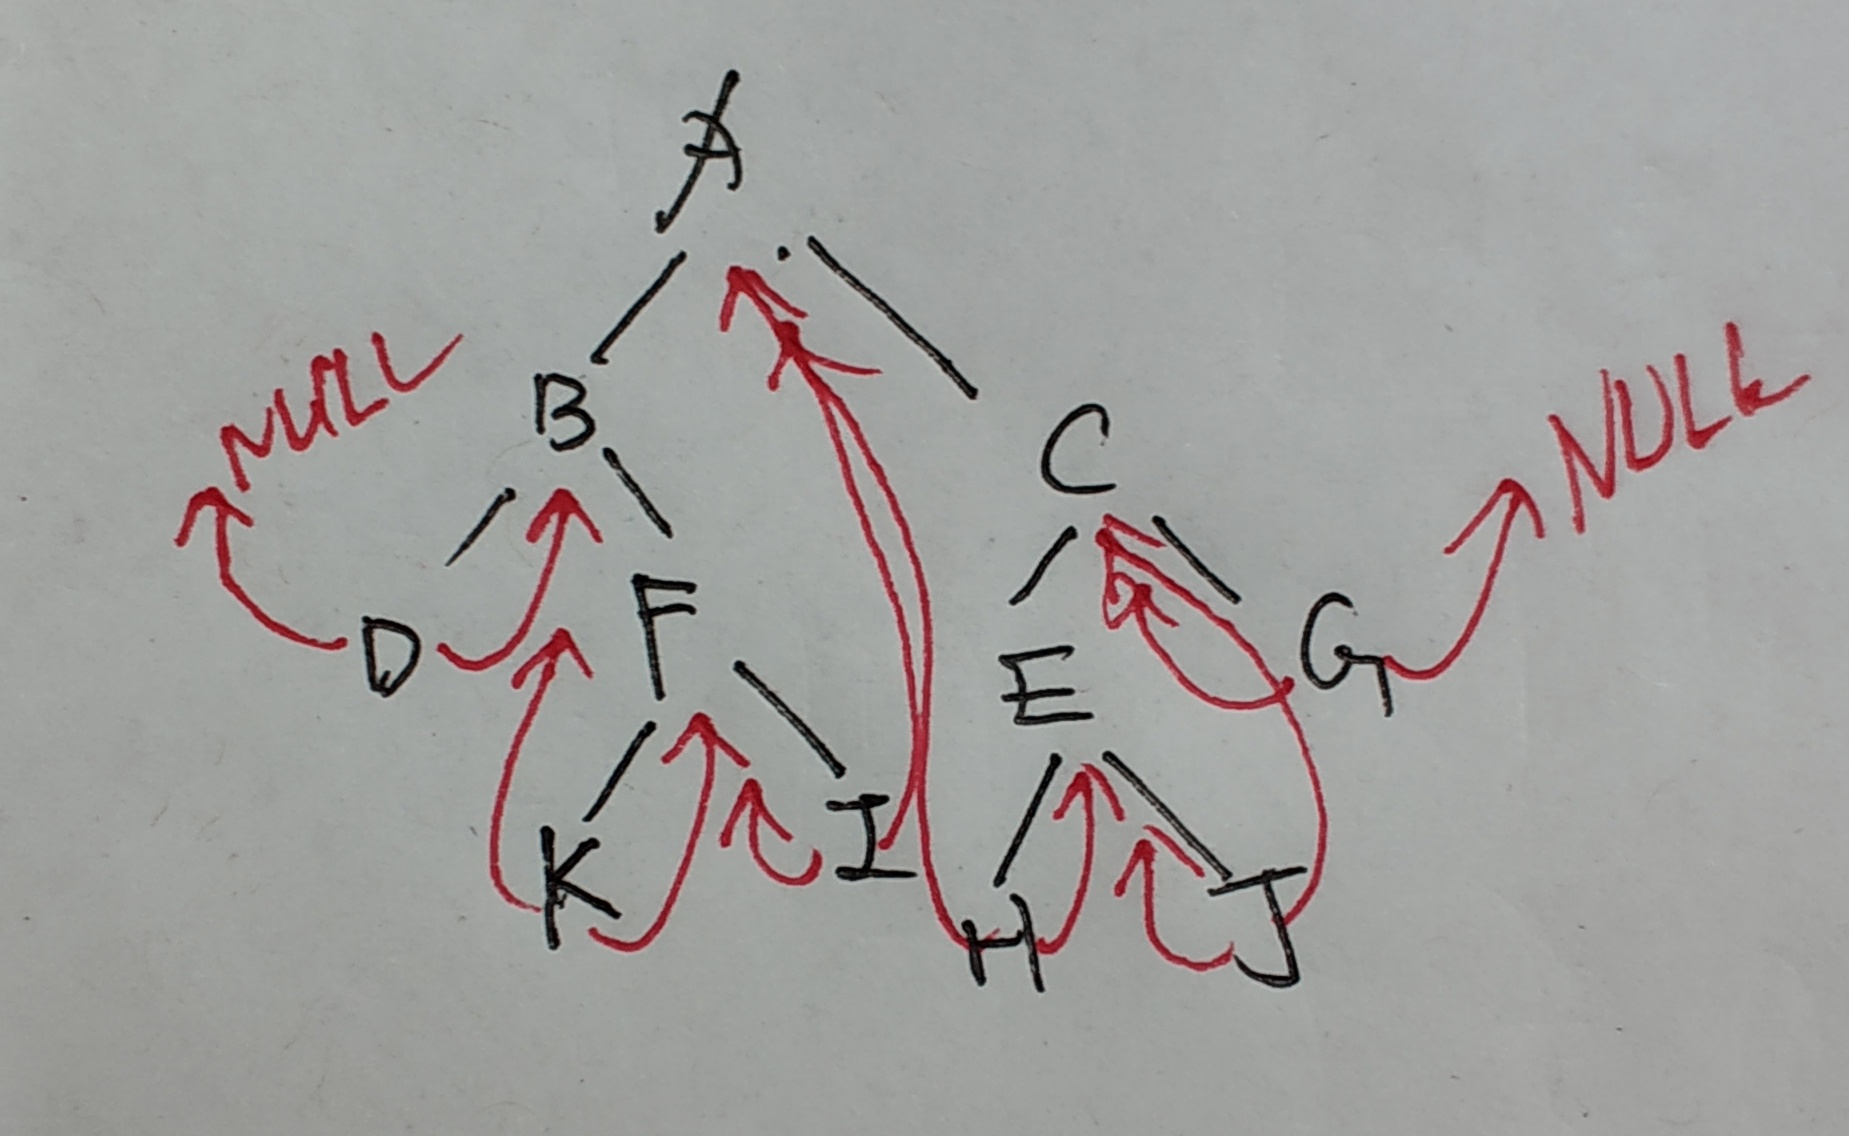
\includegraphics[scale=0.3]{example/chapter2/bitree20171.png}
\end{figure}
2. 将下图所示的森林转换成一棵二叉树,并画出这棵二叉树的顺序存储结构。\newline
\begin{figure}[H]
	\centering  % 环境中的内容居中排版
	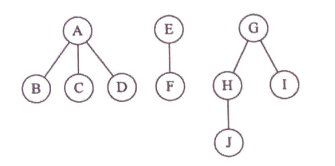
\includegraphics[scale=0.8]{example/chapter21/2019-09-10112932.png}
\end{figure} 
解:\newline

\begin{figure}[H]
	\centering  % 环境中的内容居中排版
	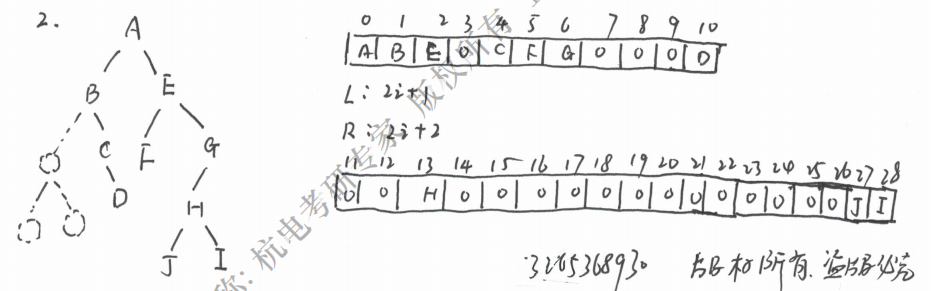
\includegraphics[scale=0.8]{example/chapter21/Annotation2019-09-10172448.png}
\end{figure} 

3. 请对下列带权无向图,按普里姆(Prim)算法求其最小生成树。(给出求解过程)\newline
\begin{figure}[H]
	\centering  % 环境中的内容居中排版
	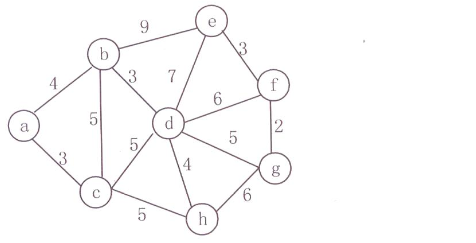
\includegraphics[scale=0.8]{example/chapter21/2019-09-10113325.png}
\end{figure} 
解:(考察Prim算法)\newline
\begin{figure}[H]
	\centering  % 环境中的内容居中排版
	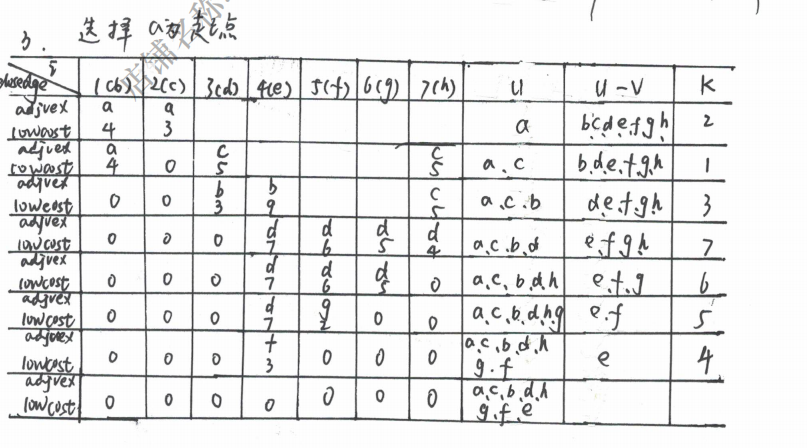
\includegraphics[scale=0.8]{example/chapter21/Annotation2019-09-10172146.png}
\end{figure} 
\begin{figure}[H]
	\centering  % 环境中的内容居中排版
	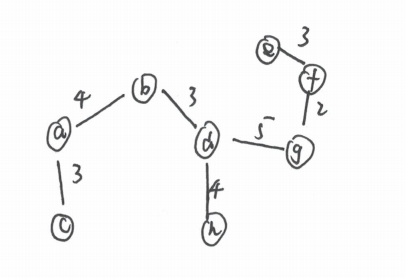
\includegraphics[scale=0.8]{example/chapter21/Annotation2019-09-10172319.png}
\end{figure}

4. 已知图G如下所示,求从顶点a到其余各顶点的最短路径。(给出求解过程)\newline
\begin{figure}[H]
	\centering  % 环境中的内容居中排版
	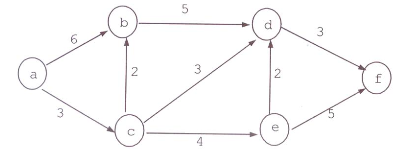
\includegraphics[scale=0.8]{example/chapter21/2019-09-10124650.png}
\end{figure} 
解:(考察DJKSTRA算法)\newline
\begin{figure}[H]
	\centering  % 环境中的内容居中排版
	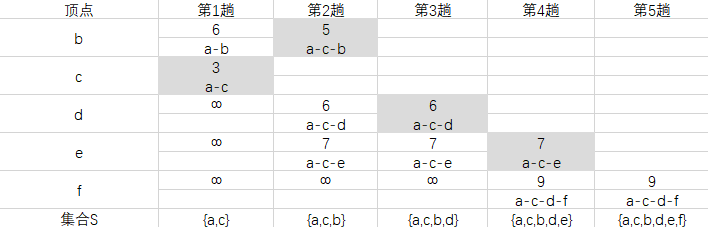
\includegraphics[scale=0.8]{example/chapter21/Annotation2019-09-10171730.png}
\end{figure} 

5. 设数据元素的关键字序列为(20, 30, 15, 45, 78, 65, 25, 60)依次插入这些元素,创建一颗平衡二叉排序树(AVL 树),请逐一画出每插入一个元素后的AVL树的形态。\newline
解:\newline
\begin{figure}[H]
	\centering  % 环境中的内容居中排版
	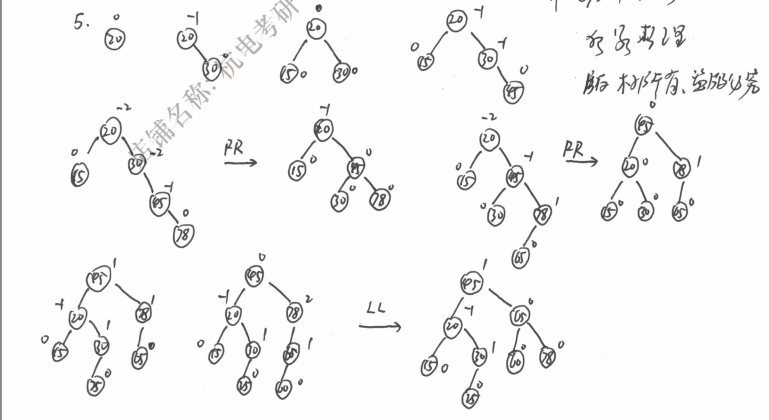
\includegraphics[scale=0.8]{example/chapter21/Annotation2019-09-10155954.png}
\end{figure} 	

六、算法设计题(本大题共三小题, 第一小题10S分, 第二小题12分, 第三小题14分, 本大题共36分)\newline
1. 二叉树的节点类型定义为\newline

\begin{lstlisting}[basicstyle=\small\ttfamily, caption={}, numbers=none]
typedef struct node{
	char data;
	struct node *lchild;
	struct node *rchild;
}NODE;
\end{lstlisting}
设计以非递归的方式实现对二叉树先序遍历的算法。\newline
解:\newline
算法设计思路: (非递归即用栈,DLR)。判断栈是否为空,或子树为空,若不为空,就访问左孩子入栈,直至左孩子为空,若左孩子为空就出战,然后访问有孩子,入栈,就这样不断的循环,直到栈空\newline
\begin{lstlisting}[basicstyle=\small\ttfamily, caption={}, numbers=none]
void PreTraverseTree(NODE *T){
	StatckNode *S;
	TreeNode *p;
	S = NULL;
	p = T;
	S = InitStack(S);
	
	if(p == NULL){
		printf("ERROR");
		return;
	}
	while(p ||!StackEmpt(S)){
		if(p){
			StackPush(S, p);
			printf("%c", p->data);
			p = p -> leftchild;
		}
		else{
			StackPop(S,p);
			p = p->rightchild;
		}
	}
	free(S);
}
\end{lstlisting}
\begin{lstlisting}[basicstyle=\small\ttfamily, caption={}, numbers=none]
#include<iostream>
#include<stack>
using namespace std;

typedef struct node {
	char data;
	struct node *lchild;
	struct node *rchild;
}NODE;


void PreTraverseTree(NODE *T) {
	stack<NODE*> S;
	NODE *p;
	p = T;
	
	if (p == NULL) {
		printf("ERROR");
		return;
	}
	while (p || !(S.empty())) {
		if (p) {
			S.push(p);
			printf("%c", p->data);
			p = p->lchild;
		}
		else {
			p = S.top();
			S.pop();
			p = p->rchild;
		}
	}
}

int main() {
	// 自己单间构造一棵树
	NODE *N[10];
	for (int i = 0; i < 6; i++) {
		N[i] = (NODE *)malloc(sizeof(NODE));
		N[i]->data = 'a' + i; N[i]->lchild = NULL; N[i]->rchild = NULL;
	}
	N[0]->lchild = N[1]; N[0]->rchild = N[2];
	N[1]->lchild = N[3]; N[1]->rchild = N[4];
	N[2]->rchild = N[5];
	
	//先序遍历的非递归算法
	PreTraverseTree(N[0]);
	system("pause");//abdecf
}
\end{lstlisting}
2. 假设待排序的n个元素存放在数据a[1],......,a[n]中,利用堆排序算法对n个元素进行升序排序。\newline
1) 请描述堆排序算法步骤;\newline
2) 写出堆排序的代码; \newline
解:\newline
算法设计思路:\newline
1.首先构建大顶堆\newline
2.输出大顶堆的最上面的元素,然后把最后一个元素放到最上面后删掉最后一个元素。直到只有一个元素为止。\newline
\begin{lstlisting}[basicstyle=\small\ttfamily, caption={}, numbers=none]
void BuildMinHeap(ElemType A[], int len){
	for(int i=len/2; i>0; i--){
		AjustDown(A,i,len);
	}
}

void AdjustDown(ElemType A[],int k, int len){
	A[0] = A[k];
	for(int i=2*k; i<=len; i=i*2){
		// 取两个子节点的最小值 
		if(i<len && A[i+1] < A[i]){
			i++;
		}
		if(A[i] >= A[0]) break;// 子节点的值比父节点的值要大那么,结束调整 
		else{//否则不符合小根堆的条件,那么把,子节点和父节点相互交换。接着向下调整。 
			A[k] = A[i];
			k = i;
		}
	}
	A[k] = A[0];
} 
void HeapSort(ElemType A[],int len){
	//首先建立小根堆
	BuildMinHeap(A,len); 
	for(i = len; i>1; i--){// 不使用第0个元素
		Swap(A[i],A[1]);
		printf("%d",A[i]);
		AdjustDown(A,1,i-1); 
	} 
}
\end{lstlisting}



3. 采用邻接表存储结构, 编写一个判别无向图中任意给定的两个顶点之间是否存在一条长度为K的简单路径的算法。注:简单路径是指其顶点序列中不含有重现的顶点。\newline
QU: 什么方法??
\begin{lstlisting}[basicstyle=\small\ttfamily, caption={}, numbers=none]
// 采用邻接表存储结构, 编写一个判别无向图中任意给定的两个顶点之间是否存在一条长度为K的简单路径的算法。
// 注:简单路径是指其顶点序列中不含有重现的顶点。
#include <iostream>
bool res = false;

bool findK(int **a, bool *visited, int n, int op, int ed, int k) {
	visited[op] = true;
	for (int i = 0; i < n; i++) {
		//找出OP的邻接点
		if (a[op][i] == 1 && visited[i] == false) {
			if (i == ed) {
				if (0 == k - 1)//遍历完毕
				return true;
				else
				continue;
			}
			res = res | findK(a, visited, n, i, ed, k - 1);//从i开始遍历
		}
	}
	visited[op] = false;
	return res;
}


int main()
{
	//初始化无向图,请无视
	int n = 5;//n * n 的矩阵
	int **a = (int **)malloc(sizeof(int *) * n);
	for (int i = 0; i < n; i++) {
		a[i] = (int *)malloc(sizeof(int) * n);// a 就是邻接矩阵
	}
	bool * visited = (bool *)malloc(sizeof(bool) * n);
	for (int i = 0; i < n; i++) {
		for (int j = 0; j < n; j++) {
			if (i != j) {
				if (i <= j)
				a[i][j] = rand() % 2;
				else
				a[i][j] = a[j][i];
			}
			else {
				a[i][i] = -1;
			}
		}
	}
	//输出无向图
	for (int i = 0; i < n; i++) {
		for (int j = 0; j < n; j++) {
			printf("%d ", a[i][j]);
		}
		printf("\n");
	}
	int op = 0;
	int ed = 0; 
	int k = 0; 
	while (scanf("%d%d%d", &op, &ed, &k) != EOF) {
	for (int i = 0; i < n; i++) {
		visited[i] = false;
	}
	res = false;
	printf("%d\n", findK(a, visited, n, op, ed, k));
}
}
\end{lstlisting}
